% !TEX program = pdflatex
\documentclass[aspectratio=169,10pt]{beamer}

% --------------------
% Theme / Colors
% --------------------
\usetheme{Madrid}
\usecolortheme{dolphin}
\usefonttheme{professionalfonts}

\definecolor{AccentBlue}{HTML}{1F77B4}
\definecolor{AccentOrange}{HTML}{FF7F0E}
\definecolor{Dark}{HTML}{1B1F23}
\definecolor{LightBG}{HTML}{F7F8FA}

\setbeamercolor{title}{fg=AccentBlue}
\setbeamercolor{frametitle}{fg=AccentBlue, bg=LightBG}
\setbeamercolor{structure}{fg=AccentBlue}
\setbeamercolor{block title}{bg=AccentBlue!10, fg=Dark}
\setbeamercolor{block body}{bg=LightBG, fg=Dark}
\setbeamercolor{itemize item}{fg=AccentOrange}
\setbeamercolor{itemize subitem}{fg=AccentOrange}

\setbeamertemplate{navigation symbols}{}
\setbeamertemplate{caption}[numbered]

% Simple footline with slide number
\setbeamertemplate{footline}{%
  \leavevmode%
  \hbox{%
  \begin{beamercolorbox}[wd=.9\paperwidth,ht=2.5ex,dp=1.0ex,left]{author in head/foot}%
    \hspace{0.8em}{\scriptsize \insertshorttitle}\hfill
  \end{beamercolorbox}%
  \begin{beamercolorbox}[wd=.1\paperwidth,ht=2.5ex,dp=1.0ex,center]{date in head/foot}%
    {\scriptsize \insertframenumber/\inserttotalframenumber}
  \end{beamercolorbox}}%
  \vskip0pt%
}

% --------------------
% Packages
% --------------------
\usepackage[T1]{fontenc}
\usepackage{lmodern}
\usepackage{microtype}
\usepackage{graphicx}
\usepackage{booktabs}
\usepackage{amsmath}
\usepackage{hyperref}
\usepackage{multimedia} % for \movie (often opens external viewer)
\usepackage{tikz}
\usetikzlibrary{arrows.meta, positioning}

% Speaker notes (optional)
\usepackage{pgfpages}
% Uncomment for presenter view (notes on 2nd screen):
% \setbeameroption{show notes on second screen=right}

% --------------------
% Helpers
% --------------------
\newcommand{\tightlist}{\setlength{\itemsep}{3pt}\setlength{\parskip}{0pt}}
\newcommand{\emphblue}[1]{\textcolor{AccentBlue}{\textbf{#1}}}
\newcommand{\emphorange}[1]{\textcolor{AccentOrange}{\textbf{#1}}}

% \title[MERL Internship Intro]{Self-Introduction \& Research Portfolio}
\title[Internship at AaltoML research group]{Self-Introduction \& Research Portfolio}
% \subtitle{Interview slides (Summer 2026)\;\;\textbullet\;\; Physical Reasoning with Digital Twins \& Instructional Video Generation}
\author{Viacheslav (Slava) Iablochnikov}
\institute{M.Sc. Computer Vision, MBZUAI \;\;|\;\; B.Sc. Physics, HSE}
\date{\today}

% Update this path if you move assets
\newcommand{\assetdir}{imgs_for_cv_presentation}

\begin{document}

% --------------------
% Title
% --------------------
\begin{frame}[plain]
  \vspace{-0.6cm}
  \begin{columns}[T,totalwidth=\textwidth]
    \begin{column}{0.62\textwidth}
      \titlepage
      \vspace{-0.2cm}
      {\small\color{Dark}Email: \href{mailto:slavawertlon@gmail.com}{slavawertlon@gmail.com} \;\textbullet\; Abu Dhabi, UAE}
    \end{column}
    \begin{column}{0.38\textwidth}
      \vspace{0.4cm}
      \centering
      \includegraphics[width=0.33\linewidth]{\assetdir/01_Logo_HSE_full_eng_CMYK.pdf}\\[0.5em]
      \includegraphics[width=1.0\linewidth]{\assetdir/mbzuai_logo_v2.png}
    \end{column}
  \end{columns}

\note{Opening (15--20s): name + current program, then 1 line about your research focus (generative video + reasoning). Mention you tailored the last part to MERL's \"Physical Reasoning with Digital Twins\" and \"Instructional Video Generation\" projects.}
\end{frame}

% --------------------
% Agenda
% --------------------
\begin{frame}{Roadmap}
\begin{itemize}
  \item \emphblue{Background}: Relevant courses, BSc thesis in scientific ML (diffusion for astronomy), and projects done during studies: adversarial robustness, face swapping, culturally-aware T2I
  \item \emphblue{MSc in CV}: current work on diffusion acceleration, physically-informed video diffusion.
  % \item \emphblue{Career goals and fit for NTU fellowship}: my motivation and how these connect to chosen projects.
  % how these connect to \emphorange{physical reasoning with digital twins} and \emphorange{instructional video generation}.
\end{itemize}

\note{Set expectations: ~10--12 minutes + Q\&A. Suggest you can dive deeper into any project if they ask.}
\end{frame}

% --------------------
% BSc Slide 1
% --------------------
\begin{frame}{B.Sc. Physics at National Research University "Higher School of Economics" \hfill \includegraphics[height=0.45cm]{\assetdir/01_Znak_HSE_CMYK.pdf}}
% \framesubtitle{Core coursework + thesis problem}

\begin{columns}[T,totalwidth=\textwidth]
\begin{column}{0.57\textwidth}
\emphblue{\emphorange{GPA: 8.33}/10.00; Core courses (selected)}
\begin{itemize}\tightlist
  \item Linear algebra, calculus, probability \& statistics, differential equations
  \item Optimization, machine learning, deep learning
  \item Data structures \& algorithms
\end{itemize}

\vspace{0.4em}
\emphblue{Bachelor thesis:} \emphorange{Diffusion models for astronomical image differencing}
\begin{block}{Problem in one sentence}
Given two sky survey images of the same field (different time/instrument), produce a \emphorange{clean difference image} to detect transient events (new stars/supernovae/etc.) with calibrated uncertainty.
\end{block}
\end{column}

\begin{column}{0.43\textwidth}
\centering
\includegraphics[width=\linewidth]{\assetdir/DiffDiff_result_2_example.png}
\vspace{0.2em}
\scriptsize Diffusion intuition (forward noise \& reverse denoising)
\end{column}
\end{columns}

\note{Talk track: (1) you're a physics grad who pivoted to modern ML; (2) thesis is a scientific-ML pipeline; (3) highlight the key theme: \"analysis-by-synthesis\" and uncertainty-aware estimation, which connects later to digital twins.}
\end{frame}

% --------------------
% BSc Slide 2
% --------------------
% \begin{frame}{Bachelor thesis: DiffDiff: Diffusion models for astronomical image differencing; results \& takeaways}
% \begin{columns}[T,totalwidth=\textwidth]
% \begin{column}{0.58\textwidth}
% \begin{itemize}\tightlist
%   \item Built an end-to-end transient processing pipeline using a \emphblue{conditional diffusion model} (U-Net + DDPM) for difference-image generation (img2img editing).
%   \item Produced clean difference frames used for \emphblue{flux + coordinate estimation} and \emphblue{uncertainty calibration}.
%   \item Trained from scratch on simulated and real data; provides reproducible training/eval, ablations, and deployment-friendly inference
%   \item Achieved \emphorange{5.6\,\texttimes\ speedup} over an existing pipeline (manual checking and classical algos) and up to \emphorange{93\% detection accuracy}.
% \end{itemize}

% \vspace{0.4em}
% % \begin{block}{Why it matters for MERL}
% % This is a concrete example of \emphorange{model-based reasoning}: infer hidden variables from observations by combining a learned model with a structured objective.
% % \end{block}
% \end{column}
% \begin{column}{0.42\textwidth}
% \centering
% \includegraphics[width=0.88\linewidth]{\assetdir/unet_v2.png}
% \vspace{0.2em}
% \includegraphics[width=\linewidth]{\assetdir/DiffDiff_result_example.png}
% \vspace{0.1em}
% \scriptsize Example: reference / science / predicted difference
% \end{column}
% \end{columns}

% \note{Hit the numbers quickly (speedup, accuracy). Then explicitly connect: digital twins also rely on estimation (states/params) using models + measurements.}
% \end{frame}

% --------------------
% Project 1: VK
% --------------------
% \begin{frame}{Research Intern (VK Company): adversarial robustness for multimodal models}
% \begin{columns}[T,totalwidth=\textwidth]
% \begin{column}{0.6\textwidth}
% \begin{itemize}\tightlist
%   \item Investigated adversarial attacks against the \emphblue{image retrieval} and \emphblue{VLM} systems.
%   \item Implemented and evaluated \emphblue{patch attacks} for CLIP / SigLIP / LLaVA-family models and video retrieval.
%   \item The new proposed attack variants achieve up to an \emphorange{86\% success rate} in forcing models to generate restricted content.
%   \item Outcome: \emphorange{\href{https://arxiv.org/abs/2412.01725}{arXiv preprint}} and a better understanding of \emphblue{model failure modes, safety, and evaluation}.
% \end{itemize}

% % \vspace{0.4em}
% % \begin{block}{Transferable to MERL}
% % Physical reasoning systems need \emphorange{robust perception and reliable evaluation}; I bring tooling for stress-testing multimodal pipelines.
% % \end{block}
% \end{column}
% \begin{column}{0.4\textwidth}
% \begin{center}
% % \includegraphics[height=0.4cm]{\assetdir/vk_logo_raster.png}\\[0.1em]
% \includegraphics[width=0.75\linewidth]{\assetdir/arc_attacks.png}\\[0.3em]
% \includegraphics[width=0.6\linewidth]{\assetdir/adversarial_attacks_example_v3.png}\\[0.3em]
% % \vspace{0.1em}
% \scriptsize Training pipeline and learned adversarial patches.
% \end{center}
% \end{column}
% \end{columns}

% \note{Pitch this as \"robustness research\" rather than \"breaking models\". Emphasize careful evaluation, threat models, and reproducibility.}
% \end{frame}

% --------------------
% Project 3: ISSAI
% --------------------
% \begin{frame}{Research Intern (ISSAI): culturally-aware text-to-image diffusion}
% \begin{columns}[T,totalwidth=\textwidth]
% \begin{column}{0.55\textwidth}
% \begin{itemize}\tightlist
%   \item Goal: improve \emphblue{prompt adherence} and \emphblue{cultural fidelity} for Kazakh imagery from multilingual prompts.
%   \item Built a targeted prompt--image corpus and trained LoRAs for Lumina2 t2i model with \texttt{diffusers}.
%   \item Full fine-tuning improved a multi-concept score from \emphorange{53.6 $\rightarrow$ 88.29}.
% \end{itemize}

% \vspace{0.4em}
% \begin{block}{Relevance}
% Strong at \emphorange{data curation + controlled fine-tuning} $\rightarrow$ essential for domain-specific fields.
% \end{block}
% \end{column}
% \begin{column}{0.42\textwidth}
% \centering
% \includegraphics[height=0.75cm]{\assetdir/issai_logo_raster.png}\\[0.5em]
% \includegraphics[width=\linewidth]{\assetdir/issai_example_1.png}\\[0.3em]
% \includegraphics[width=\linewidth]{\assetdir/issai_example_2.png}
% \end{column}
% \end{columns}

% \note{Emphasize: (1) you can build a dataset and training pipeline quickly; (2) you think about evaluation. If asked about the score: describe it as an internal / model-based metric you used in the project.}
% \end{frame}


% --------------------
% MSc slide
% --------------------
\begin{frame}{M.Sc. in Computer Vision (MBZUAI) \hfill \includegraphics[height=0.8cm]{\assetdir/mbzuai_logo_v2.png}}
\framesubtitle{Coursework \& research interests}

\begin{columns}[T,totalwidth=\textwidth]
\begin{column}{0.5\textwidth}
\emphblue{\emphorange{GPA: 3.73}/4.00; PhD-level coursework}
\begin{itemize}\tightlist
  \item Advanced Machine Learning
  \item Advanced Distributed \& Parallel ML Systems
  \item Sequential Decision Making
  \item Advanced Topics in Vision \& Language
\end{itemize}

\vspace{0.4em}
\emphblue{Research interests}
\begin{itemize}\tightlist
  \item Generative models for image/video (diffusion, DiT/MMDiT)
  \item Vision-language models \& multimodal reasoning
  \item Scientific ML / physically grounded generation
  \item Efficient training/inference
\end{itemize}
\end{column}

\begin{column}{0.48\textwidth}
\begin{block}{Throughline}
I like problems where we combine \emphorange{strong inductive biases} (physics/geometry/3D) with \emphorange{world models} (diffusion, VLMs, VLAs) to reason about dynamics.
\end{block}

\vspace{0.3em}
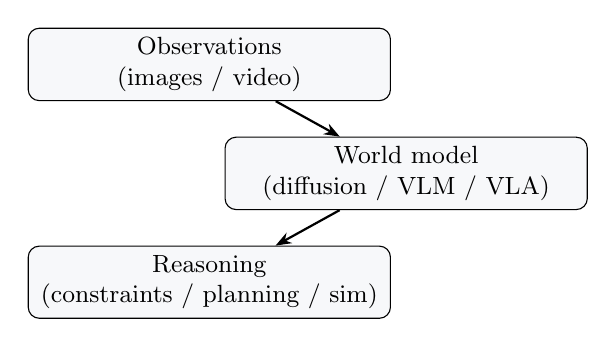
\begin{tikzpicture}[every node/.style={font=\small}, node distance=0.45cm]
\node[draw,rounded corners,fill=LightBG,align=center,minimum width=4.6cm] (obs) {Observations\\(images / video)};
\node[draw,rounded corners,fill=LightBG,align=center,below=of obs,xshift=2.5cm,minimum width=4.6cm] (model) {World model\\(diffusion / VLM / VLA)};
\node[draw,rounded corners,fill=LightBG,align=center,below=of model,xshift=-2.5cm,minimum width=4.6cm] (reason) {Reasoning\\(constraints / planning / sim)};

\draw[-{Stealth[length=2mm]},thick] (obs) -- (model);
\draw[-{Stealth[length=2mm]},thick] (model) -- (reason);
\end{tikzpicture}


\end{column}
\end{columns}

\note{Keep it high-level. The last line is your narrative: observations $\rightarrow$ model $\rightarrow$ reasoning/action. That sets up physical reasoning with digital twins.}
\end{frame}

% --------------------
% Project 4: Acceleration
% --------------------
% \begin{frame}{MBZUAI: accelerating diffusion inference (work in progress)}
% \begin{columns}[T,totalwidth=\textwidth]
% \begin{column}{0.62\textwidth}
% \begin{itemize}\tightlist
%   \item Profiling transformer-based diffusion backbones (DiT / MMDiT) on multi-GPU clusters.
%   \item Exploring \emphblue{KV caching / activation reuse} and systems-level optimizations to reduce end-to-end latency.
%   \item Tooling: PyTorch profiler, Triton kernels, distributed training/inference with \texttt{accelerate}/DeepSpeed.
% \end{itemize}

% \vspace{0.4em}
% \begin{block}{Why MERL might care}
% Digital-twin reasoning loops are compute-heavy; speedups enable \emphorange{more simulation rollouts} and tighter \emphorange{interactive} workflows.
% \end{block}
% \end{column}
% \begin{column}{0.38\textwidth}
% \centering
% \includegraphics[height=0.75cm]{\assetdir/mbzuai_logo_v2.png}\\[1.0em]

% \begin{tikzpicture}[every node/.style={font=\small}]
% \node[draw,rounded corners,fill=LightBG,minimum width=3.8cm,minimum height=0.8cm] (u) {User prompt / conditioning};
% \node[draw,rounded corners,fill=LightBG,below=0.5cm of u,minimum width=3.8cm,minimum height=0.8cm] (den) {Diffusion denoising steps};
% \node[draw,rounded corners,fill=LightBG,below=0.5cm of den,minimum width=3.8cm,minimum height=0.8cm] (out) {Video / image output};
% \draw[-{Stealth[length=2mm]},thick] (u) -- (den);
% \draw[-{Stealth[length=2mm]},thick] (den) -- (out);
% \node[fill=AccentOrange!15,rounded corners,inner sep=2pt,right=0.1cm of den] {cache / reuse};
% \end{tikzpicture}
% \end{column}
% \end{columns}

% \note{Keep it honest: ongoing work. Mention anticipated venue only if you are comfortable; otherwise say \"targeting a top-tier CV venue\".}
% \end{frame}

% --------------------
% Project 5: KineMask slide 1
% --------------------
\begin{frame}{MBZUAI: physically-informed video diffusion (KineMask) --- motivation}
% \begin{columns}[T,totalwidth=\textwidth]
% \begin{column}{0.58\textwidth}
\begin{figure}
    \centering
    \includegraphics[width=1.0\linewidth]{imgs_for_cv_presentation/kinemask_example_2.png}
    % \caption{Caption}
    \label{fig:placeholder}
\end{figure}
\begin{itemize}\tightlist
  \item Problem: video diffusion models often violate basic physics (contact, collisions, object permanence).
  % \item Goal: controllable object interactions using \emphblue{kinematic/velocity priors} + \emphblue{vision-language conditioning}.
  % \item Key idea: use a \emphorange{ControlNet-style pathway} to inject motion constraints during generation.
\end{itemize}

% \vspace{0.4em}
% \begin{block}{Project page}
% \href{https://daromog.github.io/KineMask/}{daromog.github.io/KineMask/}
% \end{block}
% \end{column}
% \begin{column}{0.42\textwidth}
% \centering
% \movie[externalviewer]{\includegraphics[width=\linewidth]{\assetdir/kinemask_carrousel_milk_poster.png}}{\assetdir/kinemask_carrousel_milk.mp4}

% \vspace{0.2em}
% \scriptsize Click image to open video (fallback: play MP4 separately)
% \end{column}
% \end{columns}

\note{1 minute max across the next 3 slides. Here: show the video teaser and define the failure mode (physics). Mention this is directly aligned with physical reasoning.}
\end{frame}


% --------------------
% Project 5: KineMask slide 1.2
% --------------------
\begin{frame}{MBZUAI: physically-informed video diffusion (KineMask) --- idea}
% \begin{columns}[T,totalwidth=\textwidth]
% \begin{column}{0.58\textwidth}
\begin{figure}
    \centering
    \includegraphics[width=1.0\linewidth]{imgs_for_cv_presentation/kinemask_architecture_V2.png}
    % \caption{Caption}
    \label{fig:placeholder}
\end{figure}
\begin{itemize}\tightlist
  % \item Problem: video diffusion models often violate basic physics (contact, collisions, object permanence).
  \item Goal: controllable object interactions using \emphblue{kinematic/velocity priors} + \emphblue{vision-language conditioning}.
  \item Key idea: use a \emphorange{ControlNet-style pathway} to inject motion constraints during generation.
\end{itemize}

% \vspace{0.4em}
% \begin{block}{Project page}
% \href{https://daromog.github.io/KineMask/}{daromog.github.io/KineMask/}
% \end{block}
% \end{column}
% \begin{column}{0.42\textwidth}
% \centering
% \movie[externalviewer]{\includegraphics[width=\linewidth]{\assetdir/kinemask_carrousel_milk_poster.png}}{\assetdir/kinemask_carrousel_milk.mp4}

% \vspace{0.2em}
% \scriptsize Click image to open video (fallback: play MP4 separately)
% \end{column}
% \end{columns}

\note{1 minute max across the next 3 slides. Here: show the video teaser and define the failure mode (physics). Mention this is directly aligned with physical reasoning.}
\end{frame}

% --------------------
% Project 5: KineMask slide 2
% --------------------
% \begin{frame}{KineMask --- architecture (high level)}
% \begin{columns}[T,totalwidth=\textwidth]
% \begin{column}{0.5\textwidth}
% \begin{itemize}\tightlist
%   \item Two-stage training with synthetic renders + velocity masks.
%   \item Conditioning via \emphblue{VLM-generated descriptions} + user-provided interaction hints.
%   \item Video diffusion backbone + \emphorange{ControlNet} injects motion priors.
% \end{itemize}

% \vspace{0.4em}
% \begin{block}{What I contributed}
% Training/inference pipeline work: data curation/conditioning, mixed-precision multi-GPU training, evaluation tooling, and extending the framework for more plausible interactions with additional i2v model.
% \end{block}
% \end{column}
% \begin{column}{0.55\textwidth}
% \centering
%     \includegraphics[width=0.65\linewidth]{\assetdir/kinamask_taining.png}\\[0.3em]
%     \includegraphics[width=0.65\linewidth]{\assetdir/kinemask_inference.png}
% \end{column}
% \end{columns}

% \note{Walk through the diagram left-to-right: (1) synthetic training, (2) ControlNet/masks, (3) inference with user input + VLM. If asked: explain why velocity masks are a useful inductive bias.}
% \end{frame}

% --------------------
% Project 5: KineMask slide 3
% --------------------
\begin{frame}{KineMask --- results \& lessons for physical reasoning}
\begin{columns}[T,totalwidth=\textwidth]
\begin{column}{0.5\textwidth}
\begin{itemize}\tightlist
  \item Trained a large image-to-video pipeline (\emphorange{Wan2.2 5B i2v + ControlNet}) with end-to-end tooling.
  \item Observed better physical plausibility than strong baselines on interactions (collisions, approach trajectories).
  \item Learned how to set up \emphblue{controlled evaluations} for motion realism (failure cases, ablations).
\end{itemize}
\end{column}
\begin{column}{0.5\textwidth}
\begin{figure}
    \centering
    \includegraphics[width=0.65\linewidth]{\assetdir/kinemask_vase_example.png}
    % \caption{Caption}
    \label{fig:placeholder}
\end{figure}
\end{column}
\end{columns}

\vspace{0.4em}
% \begin{block}{Bridge to MERL: Physical Reasoning with Digital Twins}
% Digital twins provide a \emphorange{world model}; video diffusion provides a \emphorange{prior over visual dynamics}. Combining them enables \emphblue{analysis-by-synthesis}: simulate candidates, compare with observations, refine parameters/plans.
% \end{block}
\begin{block}{Project page}
\href{https://daromog.github.io/KineMask/}{daromog.github.io/KineMask/}
\end{block}


\note{This is the pivot slide. Explicitly say: \"This is why I'm excited about MERL's digital-twins internship: it's the same loop, but with a physics engine as the world model.\"}
\end{frame}

% --------------------
% MERL Context slide
% --------------------
% \begin{frame}{MERL context: \emphorange{physical reasoning} with \emphorange{digital twins}}
% \begin{columns}[T,totalwidth=\textwidth]
% \begin{column}{0.58\textwidth}
% \begin{itemize}\tightlist
%   \item \emphblue{Digital twin:} a real-time digital counterpart of a physical object/process, combining physics-based models with measurement streams.
%   \item \emphblue{Physical reasoning:} answer counterfactual questions (\"what happens if...?\") by simulating multi-body dynamics and estimating hidden parameters.
%   \item MERL mentions combining \emphorange{digital twins} with \emphorange{large vision-and-language models} for complex reasoning.
% \end{itemize}

% \vspace{0.3em}
% \begin{block}{Example blueprint (one loop)}
% \footnotesize
% \begin{itemize}\tightlist
%   \item Perception \& VLM: parse scene + propose hypotheses/constraints.
%   \item Simulator: roll out candidate futures under those hypotheses.
%   \item Scoring/estimation: compare simulated vs. observed outcomes; refine parameters/plans.
% \end{itemize}
% \end{block}
% \end{column}
% \begin{column}{0.42\textwidth}
% \centering
% \begin{tikzpicture}[node distance=0.55cm, every node/.style={font=\small}]
% \node[draw,rounded corners,fill=LightBG,align=center] (vlm) {VLM\\(code / hypotheses)};
% \node[draw,rounded corners,fill=LightBG,below=of vlm,align=center] (sim) {Physics engine\\(digital twin)};
% \node[draw,rounded corners,fill=LightBG,below=of sim,align=center] (score) {Compare \& update\\(estimation)};
% \draw[-{Stealth[length=2mm]},thick] (vlm) -- (sim);
% \draw[-{Stealth[length=2mm]},thick] (sim) -- (score);
% \draw[-{Stealth[length=2mm]},thick] (score.east) .. controls +(1.2,0.2) and +(1.2,1.2) .. (vlm.east);
% \end{tikzpicture}

% \vspace{0.4em}
% \end{column}
% \end{columns}

% \note{Demonstrate you read the MERL posting: digital twins + VLMs + physics engines. Give the 3-step loop and relate it to your DiffDiff + KineMask experience.}
% \end{frame}


% --------------------
% NTU Fit slide 1
% --------------------
% \begin{frame}{\emphorange{Why NTU Global Connect Fellowship (GCF)?}}
% \small
% \begin{itemize}\tightlist
% \item \textbf{Bridge to a PhD:} I see GCF as a focused step from my current work on generative foundations to my long-term goal of \emphorange{embodied / physics-grounded world models}.
% \item \textbf{Research immersion:} a structured, full-time research placement with \emphorange{world-leading faculty mentorship} to stress-test ideas and research fit. % ([Corporate NTU][1])
% \item \textbf{Built-in growth:} masterclasses for academic/research careers, plus feedback loops through a final \emphorange{poster presentation} and cohort discussions. % ([Corporate NTU][2])
% \item \textbf{Community \& network:} a cohort-based programme with networking and social activities to learn how different labs frame problems and run research. % ([Corporate NTU][2])
% \item \textbf{Concrete outcome:} produce a tangible research contribution by the end of the programme (poster-ready results; ideally a draft for submission).
% \end{itemize}
% \end{frame}

% --------------------
% NTU Fit slide 2
% --------------------
% \begin{frame}{\emphorange{GCF: What I Bring \& What I Aim to Gain}}
% \small
% \begin{columns}[T,onlytextwidth]
% \column{0.5\textwidth}
% \begin{block}{\textcolor{orange}{What I bring}}
% \begin{itemize}\tightlist
% \item \emphorange{Generative CV} background (diffusion for images/video) with an emphasis on controllability and temporal consistency
% \item \emphorange{Multimodal conditioning} practice (text/image prompts; VLM-style signals) for grounded generation
% \item \emphorange{Efficiency \& scale} mindset (profiling, acceleration, multi-GPU training, reproducible pipelines)
% \item \emphorange{Research rigor} (ablations, robustness checks, failure analysis; publishable framing)
% \end{itemize}
% \end{block}

% \column{0.45\textwidth}
% \begin{block}{\textcolor{orange}{What I aim to gain}}
% \begin{itemize}\tightlist
% \item \emphorange{Guided generation beyond data} (oracle/constraint-based steering; more reliable control objectives)
% \item \emphorange{Closed-loop reasoning} linking perception $\rightarrow$ planning/control for dynamic real-world settings
% \item \emphorange{Mentorship & research practice} from NTU labs, plus professional-development masterclasses % ([Corporate NTU][2])
% \item \emphorange{PhD alignment:} identify a strong supervisor match and research direction through the GCF research experience % ([Corporate NTU][2])
% \end{itemize}
% \end{block}
% \end{columns}
% \end{frame}


% --------------------
% MERL Fit slide 1
% --------------------
% \begin{frame}{How I align with \emphorange{Physical Reasoning with Digital Twins}}
% \begin{columns}[T,totalwidth=\textwidth]
% \begin{column}{0.60\textwidth}
% % \emphblue{MERL internship asks for:}
% % \begin{itemize}\tightlist
% %   \item Physics simulators (differentiable + non-differentiable), neuro-physical reasoning
% %   \item 3D CV / robotics ML, VLMs + generative AI
% % \end{itemize}

% % \vspace{0.5em}
% \emphblue{What I bring:}
% \begin{itemize}\tightlist
%   \item \emphorange{Strong foundation in physics-aware systems} with experience in computer vision and generative modeling for dynamic scenes
%   \item \emphorange{Generative video expertise} leveraging motion priors and multimodal conditioning (e.g., VLMs) exemplified by KineMask
%   \item \emphorange{Efficient systems engineering} for rapid research iteration (multi-GPU training, performance profiling, reproducible pipelines)
%   \item \emphorange{Rigorous evaluation mindset} with focus on robustness, systematic ablations, and failure analysis
%   \item \emphorange{Modern deep learning toolchain} proficiency with PyTorch and Hugging Face frameworks (\texttt{diffusers}, \texttt{transformers})
% \end{itemize}

% \end{column}

% \begin{column}{0.40\textwidth}
% \begin{figure}
%     \centering
%     \includegraphics[width=0.9\linewidth]{\assetdir/physical_reasoning_w_digital_twins.png}
%     % \caption{Enter Caption}
%     \label{fig:placeholder}
% \end{figure}


% % \begin{block}{Concrete research pitch (3 bullets)}
% % \begin{itemize}\tightlist
% %   \item Use VLMs to propose hypotheses about \emphblue{hidden physical parameters} (friction, damping, mass).
% %   \item Run a digital twin to generate candidate rollouts; score with visual + physical constraints.
% %   \item Learn a \emphblue{policy/adapter} that amortizes this search for fast test-time reasoning.
% % \end{itemize}
% % \end{block}
% \end{column}
% \end{columns}

% \note{Reference their posting: digital twins + VLMs. Then give your pitch. Keep it practical: you can implement, run sims, and iterate quickly.}
% \end{frame}

% --------------------
% MERL Fit slide 2 (Instructional Video)
% --------------------
% \begin{frame}{Fit for \emphorange{Instructional Video Generation} (optional discussion)}
% \begin{columns}[T,totalwidth=\textwidth]
% \begin{column}{0.60\textwidth}
% \begin{itemize}\tightlist
%   \item \emphorange{Video diffusion expertise} with large-scale training and temporal coherence modeling
%   \item \emphorange{Instructional video modeling} aligning multimodal prompts (text/images) with procedural video generation
%   \item \emphorange{Conditional generation skills} integrating VLMs and motion priors into video pipelines
%   % \item \emphorange{Focused motion/region modeling} techniques for clear action and task dynamics in videos
%   \item \emphorange{Research-driven mindset} design and evaluation of models aimed at publishable insights
% \end{itemize}

% \end{column}

% \begin{column}{0.40\textwidth}
% \begin{figure}
%     \centering
%     \includegraphics[width=0.9\linewidth]{\assetdir/instructural_video_generation.png}
%     % \caption{Enter Caption}
%     \label{fig:placeholder}
% \end{figure}
% % \vspace{0.4em}
% % \begin{block}{How I'd start (first 2--3 weeks)}
% % \begin{itemize}\tightlist
% %   \item Define a clean task + dataset protocol (diagrams/steps $\rightarrow$ video segments).
% %   \item Build a baseline diffusion pipeline with conditioning + metrics.
% %   \item Add controllability: structural priors, motion masks, or simulator-guided constraints.
% % \end{itemize}
% % \end{block}
% \end{column}
% \end{columns}
% \note{If they bring up the project: position yourself as \"video diffusion + controllability + evaluation\". Mention you're comfortable with text/image/diagram conditioning and can prototype quickly.}
% \end{frame}

\begin{frame}{Training-free acceleration of diffusion models}
% \begin{columns}[T,totalwidth=\textwidth]
% \begin{column}{0.58\textwidth}
\begin{figure}
    \centering
    % \includegraphics[width=1.0\linewidth]{imgs_for_cv_presentation/kinemask_architecture_V2.png}
    \includegraphics[width=0.5\linewidth]{bottleneck_sampling.png}
    % \caption{Caption}
    \label{fig:placeholder}
\end{figure}
\begin{itemize}\tightlist
  % \item Problem: video diffusion models often violate basic physics (contact, collisions, object permanence).
  \item How can we use originally trained generative models in low-dimensional spaces?
  \item Can we reuse or condition some signals from the original denoising process?
\end{itemize}

% \vspace{0.4em}
% \begin{block}{Project page}
% \href{https://daromog.github.io/KineMask/}{daromog.github.io/KineMask/}
% \end{block}
% \end{column}
% \begin{column}{0.42\textwidth}
% \centering
% \movie[externalviewer]{\includegraphics[width=\linewidth]{\assetdir/kinemask_carrousel_milk_poster.png}}{\assetdir/kinemask_carrousel_milk.mp4}

% \vspace{0.2em}
% \scriptsize Click image to open video (fallback: play MP4 separately)
% \end{column}
% \end{columns}

\note{1 minute max across the next 3 slides. Here: show the video teaser and define the failure mode (physics). Mention this is directly aligned with physical reasoning.}
\end{frame}

% --------------------
% Closing
% --------------------
\begin{frame}{Closing}
\begin{columns}[T,totalwidth=\textwidth]
\begin{column}{0.62\textwidth}
\begin{block}{Summary}
\begin{itemize}\tightlist
  \item Physics + scientific ML background $\rightarrow$ model-based estimation mindset
  \item Strong generative modeling track record (image + video diffusion)
  \item Practical engineering: multi-GPU training, profiling, reproducibility
  % \item Clear alignment with MERL: \emphorange{physical reasoning} (world models/digital twins) and \emphorange{instructional video generation}
\end{itemize}
\end{block}
\end{column}
\begin{column}{0.38\textwidth}
\centering
\vspace{0.5em}
{\Large \emphblue{Thanks!}}\\[0.6em]
% {\small Happy to dive deeper into any slide.}\\[1.0em]
\includegraphics[width=0.85\linewidth]{\assetdir/mbzuai_logo_v2.png}
\end{column}
\end{columns}

\note{End with: \"I'm happy to discuss details of KineMask / diffusion acceleration / robustness, and brainstorm directions for your digital-twin reasoning project.\"}
\end{frame}


% --------------------
% Project 2: AIRI
% --------------------
% \begin{frame}{Research Intern (AIRI \& HSE): face / hair swapping with generative models}
% \begin{columns}[T,totalwidth=\textwidth]
% \begin{column}{0.58\textwidth}
% \begin{itemize}\tightlist
%   \item Worked on identity-preserving swapping using GAN baselines (e.g., StyleGAN2, MegaFS).
%   \item Explored \emphblue{latent-space attention} (W+, FS+ spaces) and \emphblue{rotary embeddings} for better detail transfer.
%   \item Improved perceptual similarity (\emphorange{LPIPS, 40\% impr.}) and fidelity (\emphorange{FID@1k, 87\% impr.}) versus baselines.
% \end{itemize}

% \vspace{0.4em}
% \begin{block}{What I learned}
% How to design \emphorange{architecture-level inductive biases} and diagnose training instabilities in large generative models.
% \end{block}
% \end{column}
% \begin{column}{0.40\textwidth}
% \centering
% \includegraphics[height=0.7cm]{\assetdir/airi_logo_raster.png}\\[0.6em]
% \includegraphics[width=\linewidth]{\assetdir/face_swap_example.png}
% \end{column}
% \end{columns}

% \note{Keep it short: the point is generative-model intuition + architectural changes. If asked: explain inner models/latent-space editing and metrics.}
% \end{frame}

\end{document}
